\section{Virtualizzazione}
Una teconologia che permette di \textbf{astrarre l'hardware} di un computer e creare diversi ambienti di esecuzioni. Rende quindi possibile eseguire un sistema operativo come applicazione all'interno di un altro sistema.

\spacer
L'utilizzo di una macchina virtuale garantisce la completa \textbf{protezione delle risorse}, sia per la macchina virtuale che per il sistema ospitante.

La condivisione delle risorse rimane possibile, rendendo possibile la creazione di sistemi estramemente efficienti, dove le risorse di una VM in idle vengono sfruttate dalle altre.

\spacer
Dal punto di vista implementativo la macchina virtuale realizza un'\textbf{interfaccia} indistinguibile da quella di un sistema dedicato.
Le risorse del computer fisico vengono condivise dall'hypervisor o VMM (Virtual Machine Manager) che può sfruttare tutte le funzioni del sistema ospitante per creare l'illusione che ogni utente abbia il proprio sistema.


\subsubsection*{Emulazione}
Un altro aspetto della virtualizzazione è l'emulazione, ovvero la \textbf{simulazione di componenti} hardware in software.

Più in generale è possibile emulare un intero sistema operativo scritto per un'architettura diversa.

L'emulazione però viene ad un costo importante dal punto di vista delle prestazioni, non ci si può aspettare che il codice abbia le stesse performance su tutte le architetture.

\begin{figure}[H]
    \centering
    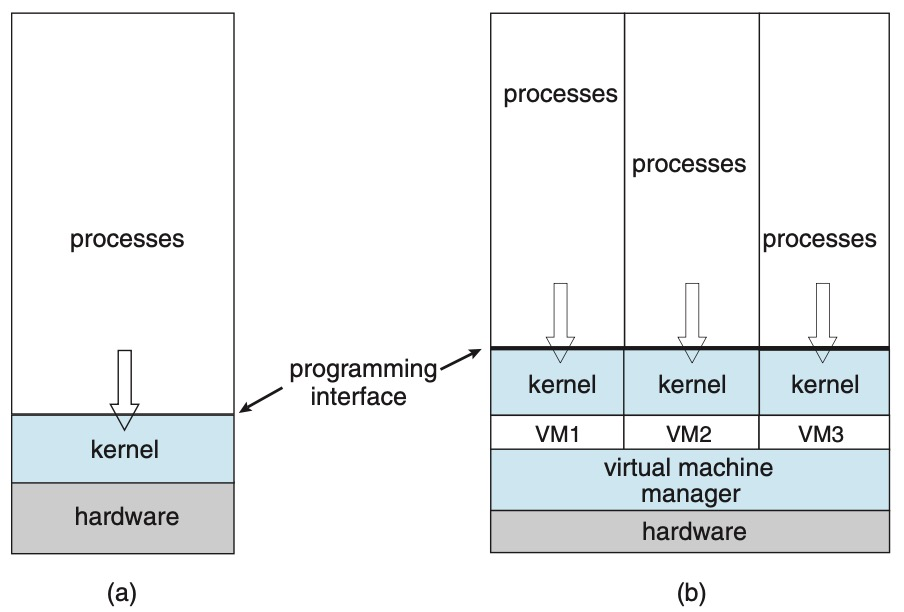
\includegraphics[width=0.4\linewidth]{assets/VMM.jpg}
    \caption{Virtual Machine Manager}
\end{figure}

\begin{note}
    \textbf{Nota di Ingegneria del Software}

    Un' applicazione delle macchine virtuali si trova proprio nello sviluppo e nel test di applicazioni, con una macchina virtuale è possibile testare l'applicazione su varie combinazioni di hardware e software.
\end{note}

\subsubsection*{Apple}
Negli ultimi anni Apple ha costruito diversi strumenti per l'emulazione, a partire dal software Rosetta 2, utilizzato per agevolare la transizione tra mac con processori intel a mac con architettura ARM.
A partire da macOS Sonoma apple ha introdotto il Game Porting Toolkit, uno strumento che permette agli sviluppatori di traddurre giochi scritti in DirectX12 a Metal 3, aumentando notevolemente le prestazioni con un minimo sforzo.
